% !TeX program = pdflatex
\documentclass[12pt,a4paper]{article}

\usepackage[margin=22mm,headheight=15pt]{geometry}
\usepackage[T1]{fontenc}
\usepackage[utf8]{inputenc}
\usepackage{lmodern}
\usepackage{graphicx}
\usepackage{amsmath,amssymb}
\usepackage{booktabs}
\usepackage{tabularx}
\usepackage{array}
\usepackage{float}
\usepackage{caption}
\usepackage{subcaption}
\usepackage{fancyhdr}
\usepackage{titlesec}
\usepackage{xcolor}
\usepackage{hyperref}
\usepackage{microtype}

\graphicspath{{figures/}}
\hypersetup{colorlinks=true,linkcolor=black,urlcolor=blue,citecolor=black}
\pagestyle{fancy}
\fancyhf{}
\lhead{Biomechanics}
\rhead{3D Motion Analysis Practical}
\cfoot{\thepage}
\titleformat{\section}{\Large\bfseries}{\thesection}{0.7em}{}
\titleformat{\subsection}{\large\bfseries}{\thesubsection}{0.7em}{}
\setlength{\parindent}{0pt}
\setlength{\parskip}{5pt}
\renewcommand{\arraystretch}{1.15}
\newcommand{\file}[1]{\texttt{\detokenize{#1}}}
\newcommand{\unit}[1]{\,\mathrm{#1}}

\begin{document}
\pagenumbering{gobble}

\begin{titlepage}
  \centering
  \vspace*{8mm}
  \IfFileExists{campus_logo.png}{
\includegraphics[width=4.2cm]{campus_logo.png}\par\vspace{7mm}}{\vspace*{10mm}}
  {\large University of Moratuwa\par}
  \vspace{15mm}
  {\large B.Sc. Engineering (Hons)\par}
  \vspace{4mm}
  {\Large\bfseries Department of Mechanical Engineering\par}
  \vspace{14mm}
  {\Huge\bfseries 3D Motion Analysis Practical Report\par}
  \vspace{5mm}
  {\LARGE Visual Motion Capture and MATLAB Kinematic Reconstruction\par}
  \vspace{4mm}
  {\large Analysis of the supplied \file{Motion2026.c3d} recording\par}
  \vfill
  \begin{tabular}{rl}
    \textbf{Module Code:} & BM3500 \\
    \textbf{Module Title:} & Biomedical Engineering Applications \\
    \textbf{Laboratory:} & Bionics Laboratory \\
    \textbf{Student Name \& Index:} & Nuwanaka W.A.S. (230449N) \\
    \textbf{Facilitators:} & Ms. E.M.A.I. Ekanayake, Mrs. N.B.N. Nuwarapaksha \\
    \textbf{Date:} & \today \\
  \end{tabular}
  \vfill
\end{titlepage}

\pagenumbering{roman}
\tableofcontents
\clearpage
\pagenumbering{arabic}
\setcounter{page}{1}

\section{Introduction}

Three-dimensional (3D) optical motion capture records the spatial trajectories of reflective markers attached to a moving subject. These trajectories can be used to describe movement, estimate linear kinematic quantities, and calculate geometric angles between segments. The Coordinate 3D (C3D) format stores motion-capture point data together with acquisition metadata in a structured binary file.

This report analyses the supplied file \file{Motion2026.c3d}. The practical used a Visual Motion Capture (VMC) system to record lower-limb marker motion and provide joint-angle outputs. The marker-coordinate and system-angle data were reconstructed and analysed in MATLAB. This report describes that workflow, summarises the VMC joint-angle results recorded in the original report draft, and separately inspects the supplied Motion2026.c3d file as a coordinate-data cross-check. The VMC-reported joint angles are treated as the primary angle result; angles calculated independently from four C3D marker trajectories are treated only as a secondary geometric check because they may use different models and conventions.

The objectives were to:
\begin{enumerate}
  \item read and verify the C3D header and point parameters;
  \item convert the recorded marker coordinates from millimetres to metres;
  \item plot marker trajectories and coordinate time series;
  \item reconstruct the VMC-provided knee and ankle angle time histories in MATLAB and calculate their range of motion and angular derivatives;
  \item use the supplied C3D coordinates as a separate check on spatial trajectories, inter-marker distances, and marker-derived geometric angles; and
  \item distinguish system-reported joint angles from secondary values calculated directly from marker coordinates.
\end{enumerate}

\section{Methods}

\subsection{C3D file and acquisition metadata}

The file was decoded as a little-endian C3D recording. The header and \texttt{POINT} and \texttt{ANALOG} parameter groups were read to obtain the point count, frame interval, coordinate units, and data-section location. \file{POINT:SCALE} is negative, indicating floating-point point records; therefore, the coordinate values were not multiplied by an integer storage scale. The \file{POINT:UNITS} parameter is \file{mm}, so coordinates were divided by 1000 to express positions in metres.

\begin{table}[H]
\centering
\caption{Metadata extracted from \file{Motion2026.c3d}.}
\label{tab:metadata}
\begin{tabularx}{\textwidth}{>{\raggedright\arraybackslash}p{0.42\textwidth}X}
\toprule
\textbf{Parameter} & \textbf{Value decoded from file} \\
\midrule
File size & 118,784 bytes (116 KiB) \\
Number of point trajectories & 4 \\
First and last frame & 1 and 1825 \\
Total number of frames & 1825 \\
Point sampling frequency & 100 Hz \\
Time between frames & 0.010 s \\
Elapsed time between first and last samples & 18.24 s \\
Point coordinate units & mm \\
Point storage scale & $-1.0$ (floating-point point data) \\
First data block & Block 4 \\
Analog channels used & 0 \\
Point labels & \file{left h}, \file{left k}, \file{left a}, \file{left f} \\
Point descriptions & left hip, left knee, left ankle-bone, left foot \\
\bottomrule
\end{tabularx}
\end{table}

The file contains four marker trajectories and no analog channels reported as used. Consequently, ground-reaction forces, recorded electromyography, and other analog signals cannot be analysed from this file. The fourth floating-point value in every point record was zero throughout the file; it was therefore not treated as a useful per-frame reconstruction-quality measure.

\subsection{Visual Motion Capture joint angles and MATLAB reconstruction}

The Visual Motion Capture system supplied the joint-angle measurements used for the main knee and ankle angle analysis. These system outputs were imported into MATLAB, where the angle records were reconstructed as time histories, plotted against time, and summarised using minimum, maximum, and range of motion (ROM). Angular velocity and acceleration were obtained from the angle-versus-time data by numerical differentiation. The angle convention is the one produced by the VMC system; the values are not redefined by applying a new dot-product calculation to the four markers in the C3D file.

For a sampled angle series $\theta(t)$, the range of motion is $\mathrm{ROM}=\theta_{\max}-\theta_{\min}$. For uniformly sampled data, central finite differences provide interior derivative estimates:
\begin{align}
\omega_i &\approx \frac{\theta_{i+1}-\theta_{i-1}}{2\Delta t},\\
\alpha_i &\approx \frac{\theta_{i+1}-2\theta_i+\theta_{i-1}}{(\Delta t)^2}.
\end{align}
Peak derivative values depend on the sampling interval and any system or MATLAB smoothing. They are interpreted as outputs of the processing workflow, not as direct measures of muscle force or joint loading.

The supplied \file{Motion2026.c3d} file contains four point trajectories and no analog angle channels. Therefore, the VMC angle series and the C3D coordinate series are treated as related but distinct data exports. The supplied file \file{VMC_joint_angles.csv} contains only the column headers and no recorded angle rows. Therefore, the summary values below are retained from the original report draft and cannot be independently recalculated from that CSV in this revision. The full VMC time history must be reconstructed from a populated angle export; it cannot be recovered from the C3D coordinates alone.

\subsection{Coordinate extraction and quality checks}

For marker $m$ at frame $n$, the position vector in metres is
\begin{equation}
\mathbf{r}_m[n] = \frac{1}{1000}
\begin{bmatrix}
X_m[n]\\Y_m[n]\\Z_m[n]
\end{bmatrix}_{\mathrm{mm}}.
\label{eq:units}
\end{equation}
The stored axis names $X$, $Y$, and $Z$ are retained as written. The file does not provide sufficient verified information to assign them anatomical meanings such as anterior--posterior or medial--lateral.

The decoded data were checked for non-finite coordinates and rows in which all three coordinates were exactly zero. None of the four markers had such rows. This basic check cannot establish tracking quality or anatomical correctness: all fourth-component values were zero, and large between-frame movements and changing inter-marker distances were found. These C3D findings are discussed as a separate coordinate-data quality check; they do not automatically invalidate the joint-angle values reported by the VMC system.

\subsection{Filtering and linear kinematics}

Numerical differentiation magnifies high-frequency coordinate noise. For descriptive derivatives, the coordinate traces were passed through a fourth-order, zero-phase Butterworth low-pass filter with a 6 Hz cutoff at the verified 100 Hz sample rate. This is an analysis choice, not a filter setting stored in the C3D file. Filtered marker positions are denoted by $\widetilde{\mathbf r}_m[n]$.

Central differences were then used for interior samples:
\begin{equation}
\mathbf{v}_m[n] \approx \frac{\widetilde{\mathbf r}_m[n+1]-\widetilde{\mathbf r}_m[n-1]}{2\Delta t},
\label{eq:velocity}
\end{equation}
\begin{equation}
\mathbf{a}_m[n] \approx \frac{\widetilde{\mathbf r}_m[n+1]-2\widetilde{\mathbf r}_m[n]+\widetilde{\mathbf r}_m[n-1]}{\Delta t^2},
\label{eq:acceleration}
\end{equation}
where $\Delta t=0.010\unit{s}$. The speed and acceleration magnitude were calculated as $v_m[n]=\|\mathbf{v}_m[n]\|$ and $a_m[n]=\|\mathbf{a}_m[n]\|$. Because the recording contains conspicuous sample-to-sample shifts, the resulting maxima are reported as numerical diagnostics rather than interpreted as valid physiological peak values.

\subsection{Inter-marker lengths and geometric angles}

Distances between adjacent labelled markers were calculated from the original recorded coordinates:
\begin{align}
L_{\mathrm{thigh}}[n] &= \|\mathbf r_H[n]-\mathbf r_K[n]\|,\\
L_{\mathrm{shank}}[n] &= \|\mathbf r_K[n]-\mathbf r_A[n]\|,\\
L_{\mathrm{foot}}[n] &= \|\mathbf r_A[n]-\mathbf r_F[n]\|.
\end{align}
Here $H$, $K$, $A$, and $F$ represent the labels left hip, left knee, left ankle-bone, and left foot, respectively. These are inter-marker distances, not independently measured anatomical segment lengths.

For a basic geometric description, the knee included angle was calculated between the vectors from the knee to the hip and from the knee to the ankle. A knee-flexion proxy was defined as $180^\circ$ minus this included angle. The ankle measure is the unsigned included angle between the ankle-to-knee vector and ankle-to-foot vector. The formulas use the filtered coordinates and the 3D dot product:
\begin{equation}
\theta = \cos^{-1}\!\left(\frac{\mathbf u\cdot\mathbf v}{\|\mathbf u\|\|\mathbf v\|}\right)\frac{180^\circ}{\pi}.
\label{eq:angle}
\end{equation}
These are simple marker-based geometric measures and are included only as a secondary comparison. They are not the primary VMC-reported joint angles. Without confirmation that the same marker model, coordinate transformation, joint-centre definitions, and angle convention were applied, a geometric angle derived from the C3D points should not be expected to match the VMC system output exactly.

\section{Results}

\subsection{Recorded marker trajectories}

The file contains trajectories for four labelled markers. Figure~\ref{fig:trajectory} shows the raw 3D paths, and Figure~\ref{fig:coordinates} shows the recorded coordinate components through time. The coordinate ranges in Table~\ref{tab:coordinates} were calculated from every decoded frame and converted from millimetres to metres.

\begin{figure}[H]
\centering
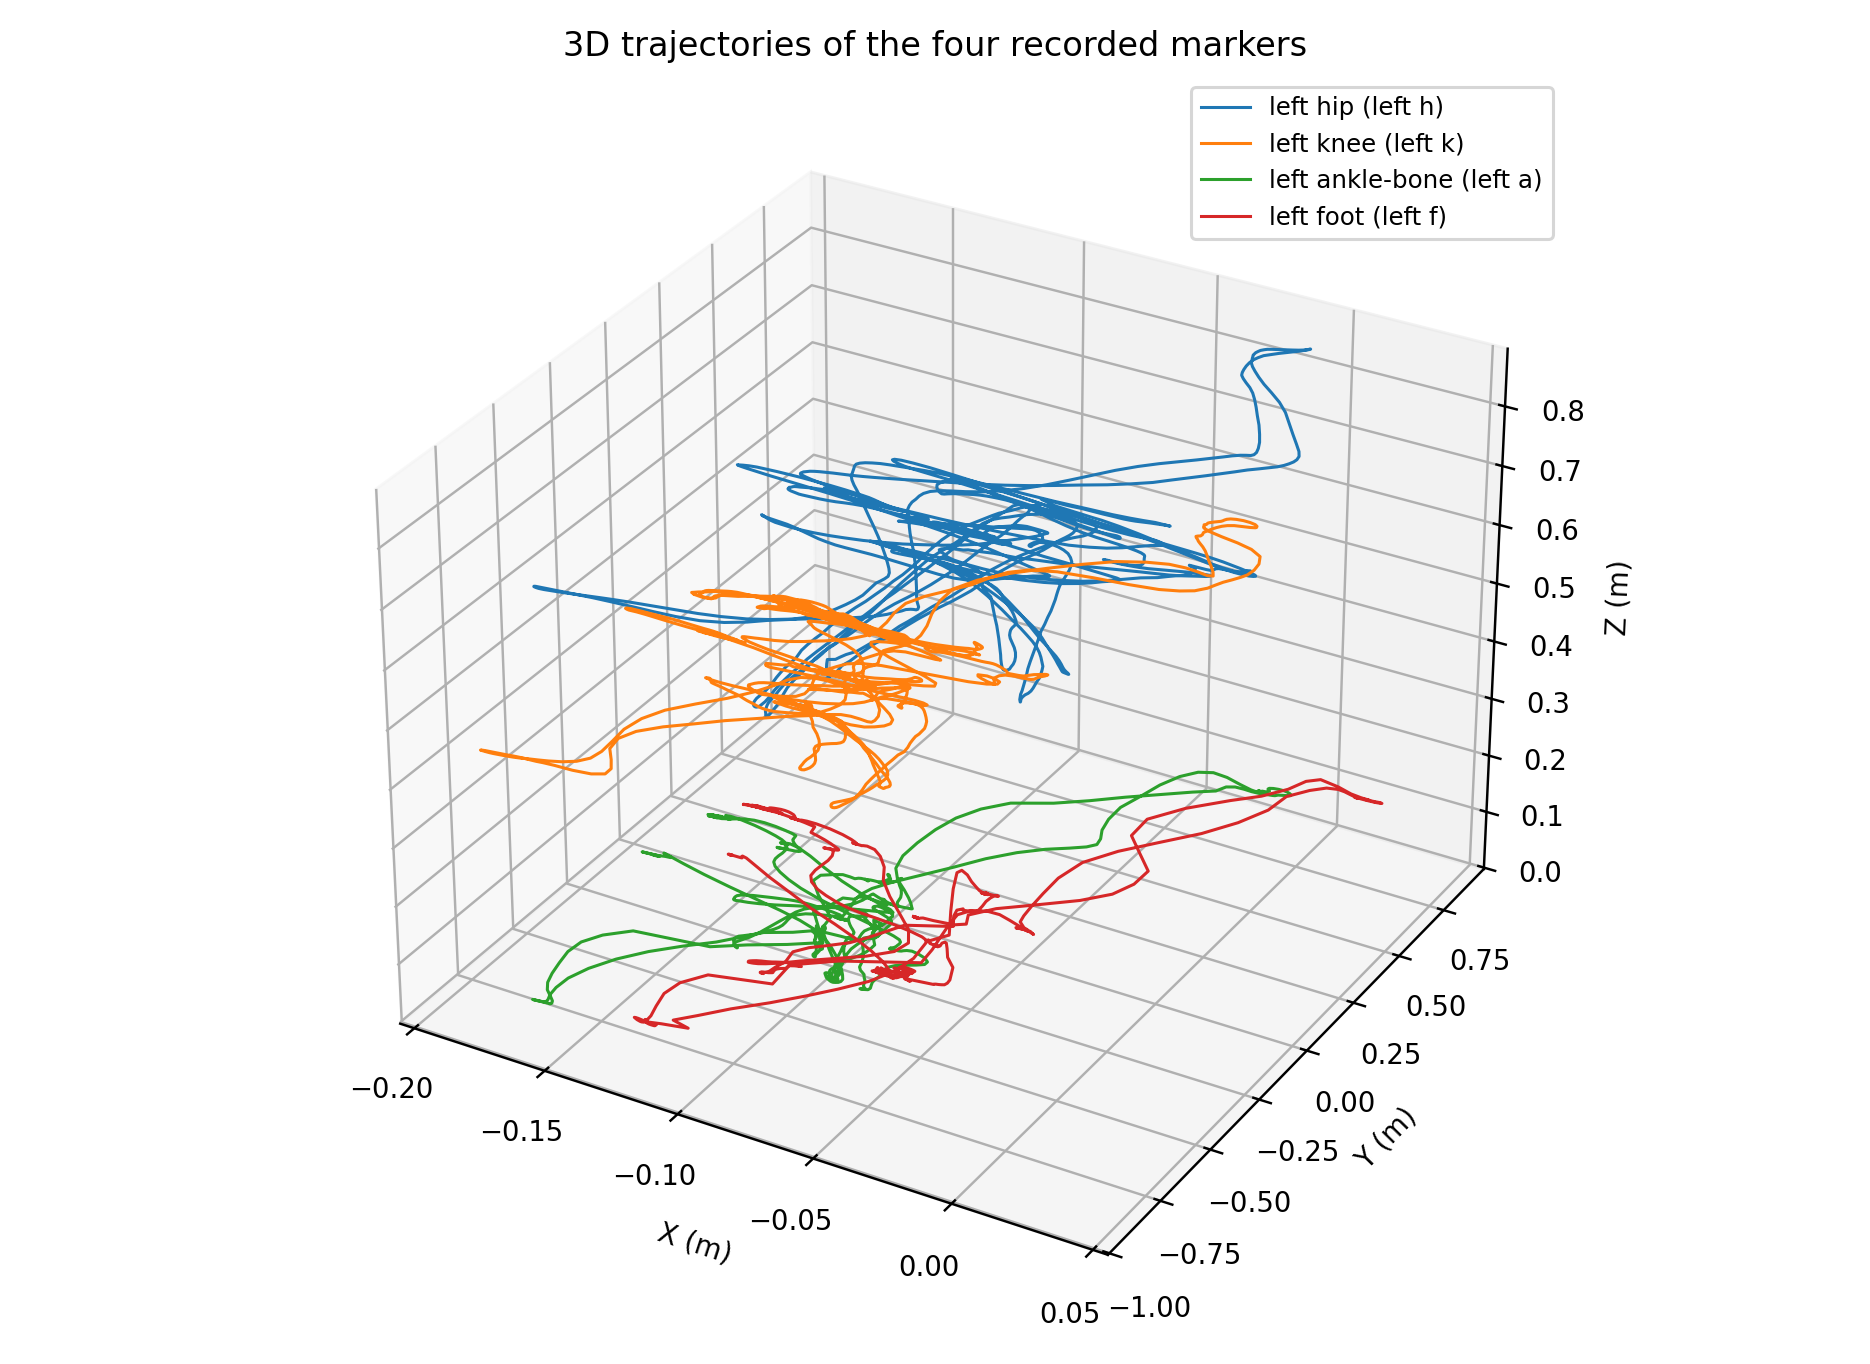
\includegraphics[width=0.88\textwidth]{marker_trajectories_3d.png}
\caption{Raw 3D trajectories for the four markers. The displayed $X$, $Y$, and $Z$ axes retain the coordinate names in the C3D file; anatomical axis directions are not inferred.}
\label{fig:trajectory}
\end{figure}

\begin{figure}[H]
\centering
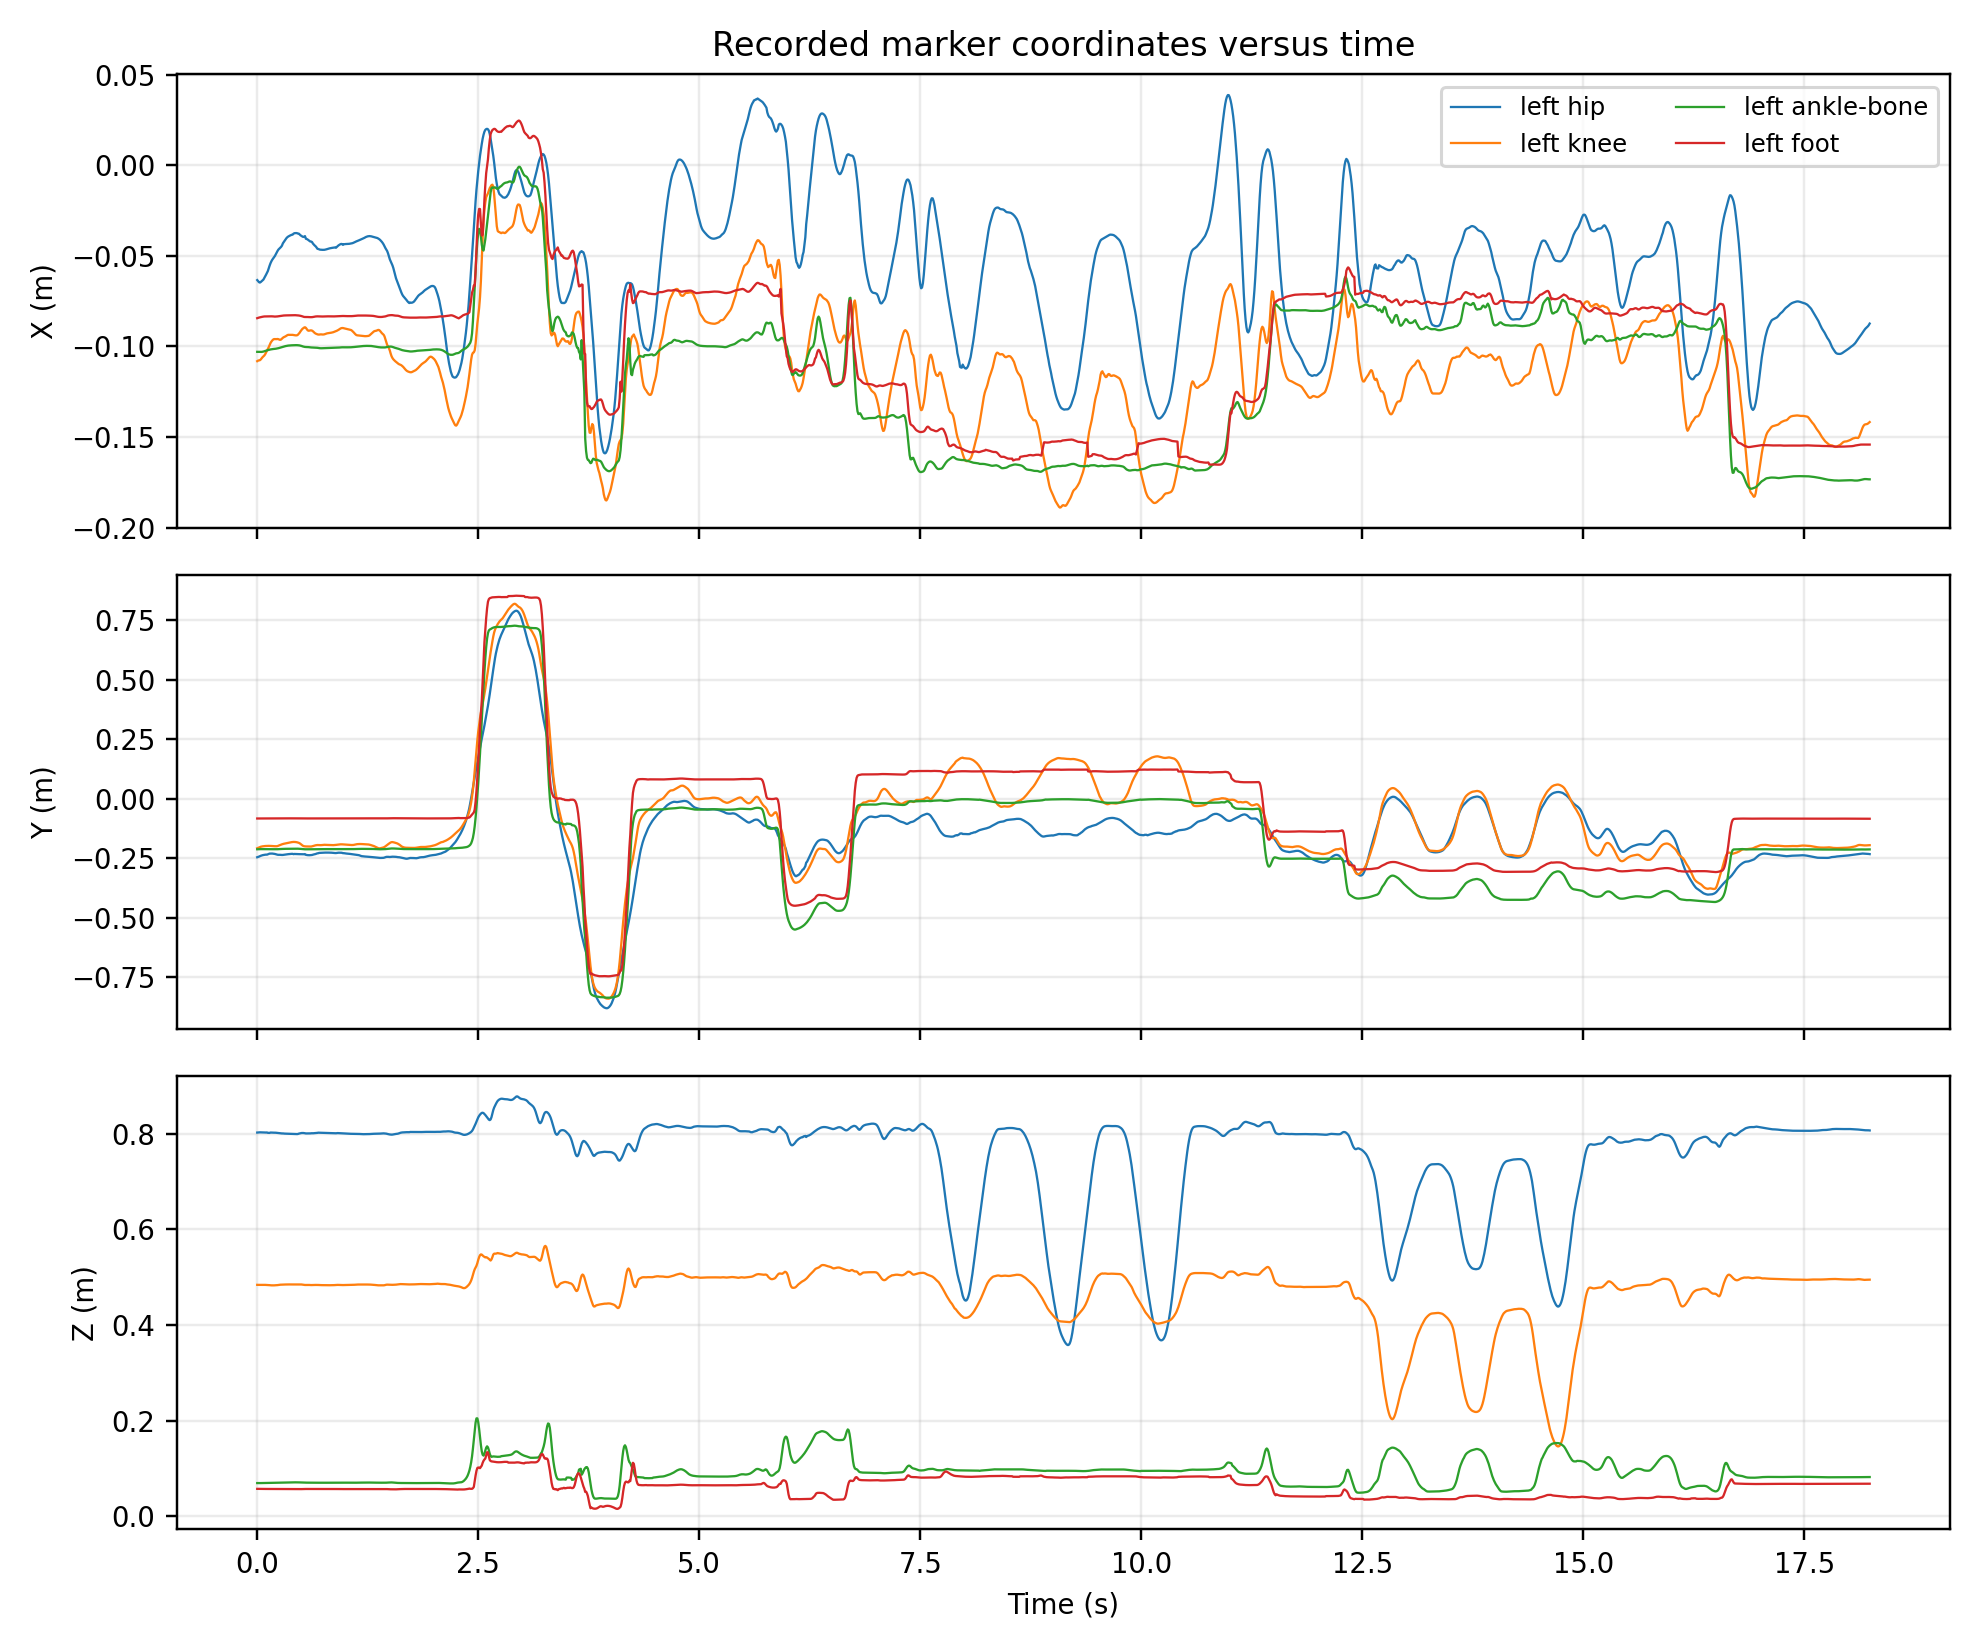
\includegraphics[width=0.95\textwidth]{marker_coordinates_time.png}
\caption{Raw $X$, $Y$, and $Z$ coordinates plotted against elapsed time. Several abrupt changes appear across multiple markers and should be reviewed against the original capture session.}
\label{fig:coordinates}
\end{figure}

\begin{table}[H]
\centering
\caption{Coordinate extrema calculated from \file{Motion2026.c3d}; values are in metres.}
\label{tab:coordinates}
\scriptsize
\setlength{\tabcolsep}{4pt}
\begin{tabular}{lrrrrrr}
\toprule
\textbf{Marker} & $X_{\min}$ & $X_{\max}$ & $Y_{\min}$ & $Y_{\max}$ & $Z_{\min}$ & $Z_{\max}$ \\
\midrule
Left hip & -0.159 & 0.039 & -0.881 & 0.790 & 0.358 & 0.878 \\
Left knee & -0.189 & -0.011 & -0.840 & 0.820 & 0.146 & 0.565 \\
Left ankle-bone & -0.179 & -0.001 & -0.836 & 0.727 & 0.037 & 0.205 \\
Left foot & -0.165 & 0.025 & -0.747 & 0.853 & 0.016 & 0.134 \\
\bottomrule
\end{tabular}
\end{table}

\subsection{Sample-to-sample changes in the C3D coordinate export}
\label{sec:quality}

The independent C3D coordinate check shows large adjacent-frame displacements at 100 Hz: 32.4 mm for the hip, 50.4 mm for the knee, 91.0 mm for the ankle marker, and 92.1 mm for the foot marker. The largest values occur at frames 335--336, 332--333, 367--368, and 327--328, respectively. These abrupt changes warrant checking the C3D export, trial boundaries, marker labels, coordinate transformations, and tracking/reconstruction settings before relying on derivatives calculated from this coordinate stream. This is a limitation of the decoded C3D point series; it should not be used on its own to dismiss the separately reported VMC angle output.

\begin{figure}[H]
\centering
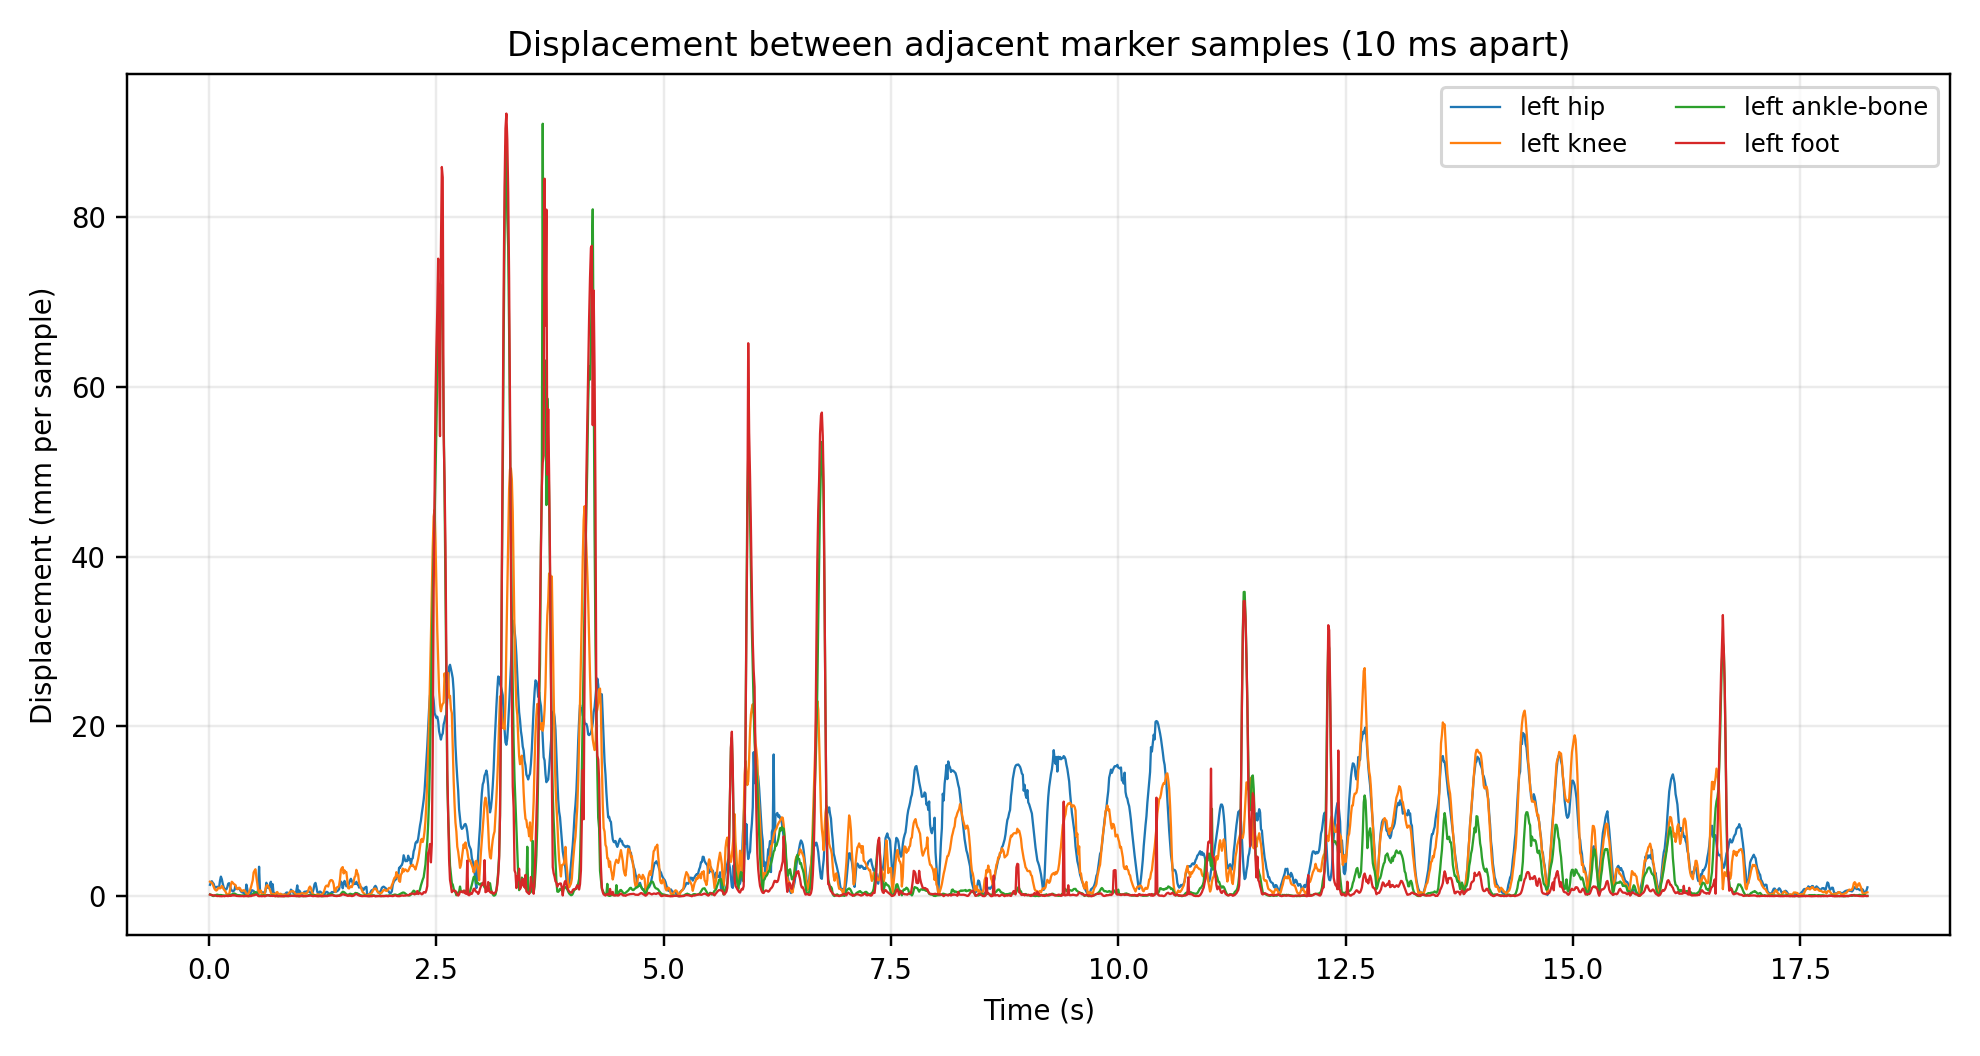
\includegraphics[width=0.92\textwidth]{framewise_displacement.png}
\caption{Euclidean displacement between adjacent samples, in millimetres per 10 ms interval. Large short-duration excursions affect several markers and are a warning against interpreting numerical velocity and acceleration peaks as physiological events.}
\label{fig:steps}
\end{figure}

No all-zero coordinate rows or non-finite XYZ values were found, but that basic check does not rule out marker swaps, reconstruction jumps, trial segmentation problems, or other tracking errors. The zero fourth components in the point records also prevent the fourth field from acting as an informative quality score in this file.

\subsection{Linear kinematic derivatives}

Figure~\ref{fig:speed} plots speed magnitudes after the stated 6 Hz low-pass filter. Descriptive values are listed in Table~\ref{tab:speed}. The peak speeds, particularly for the ankle and foot, remain unusually high because a low-pass filter cannot correct substantial trajectory shifts. These are diagnostics from the C3D coordinate stream only. They are not the velocities or accelerations of the VMC angle signals, which are calculated separately from the system-provided angle time histories in MATLAB.

\begin{figure}[H]
\centering
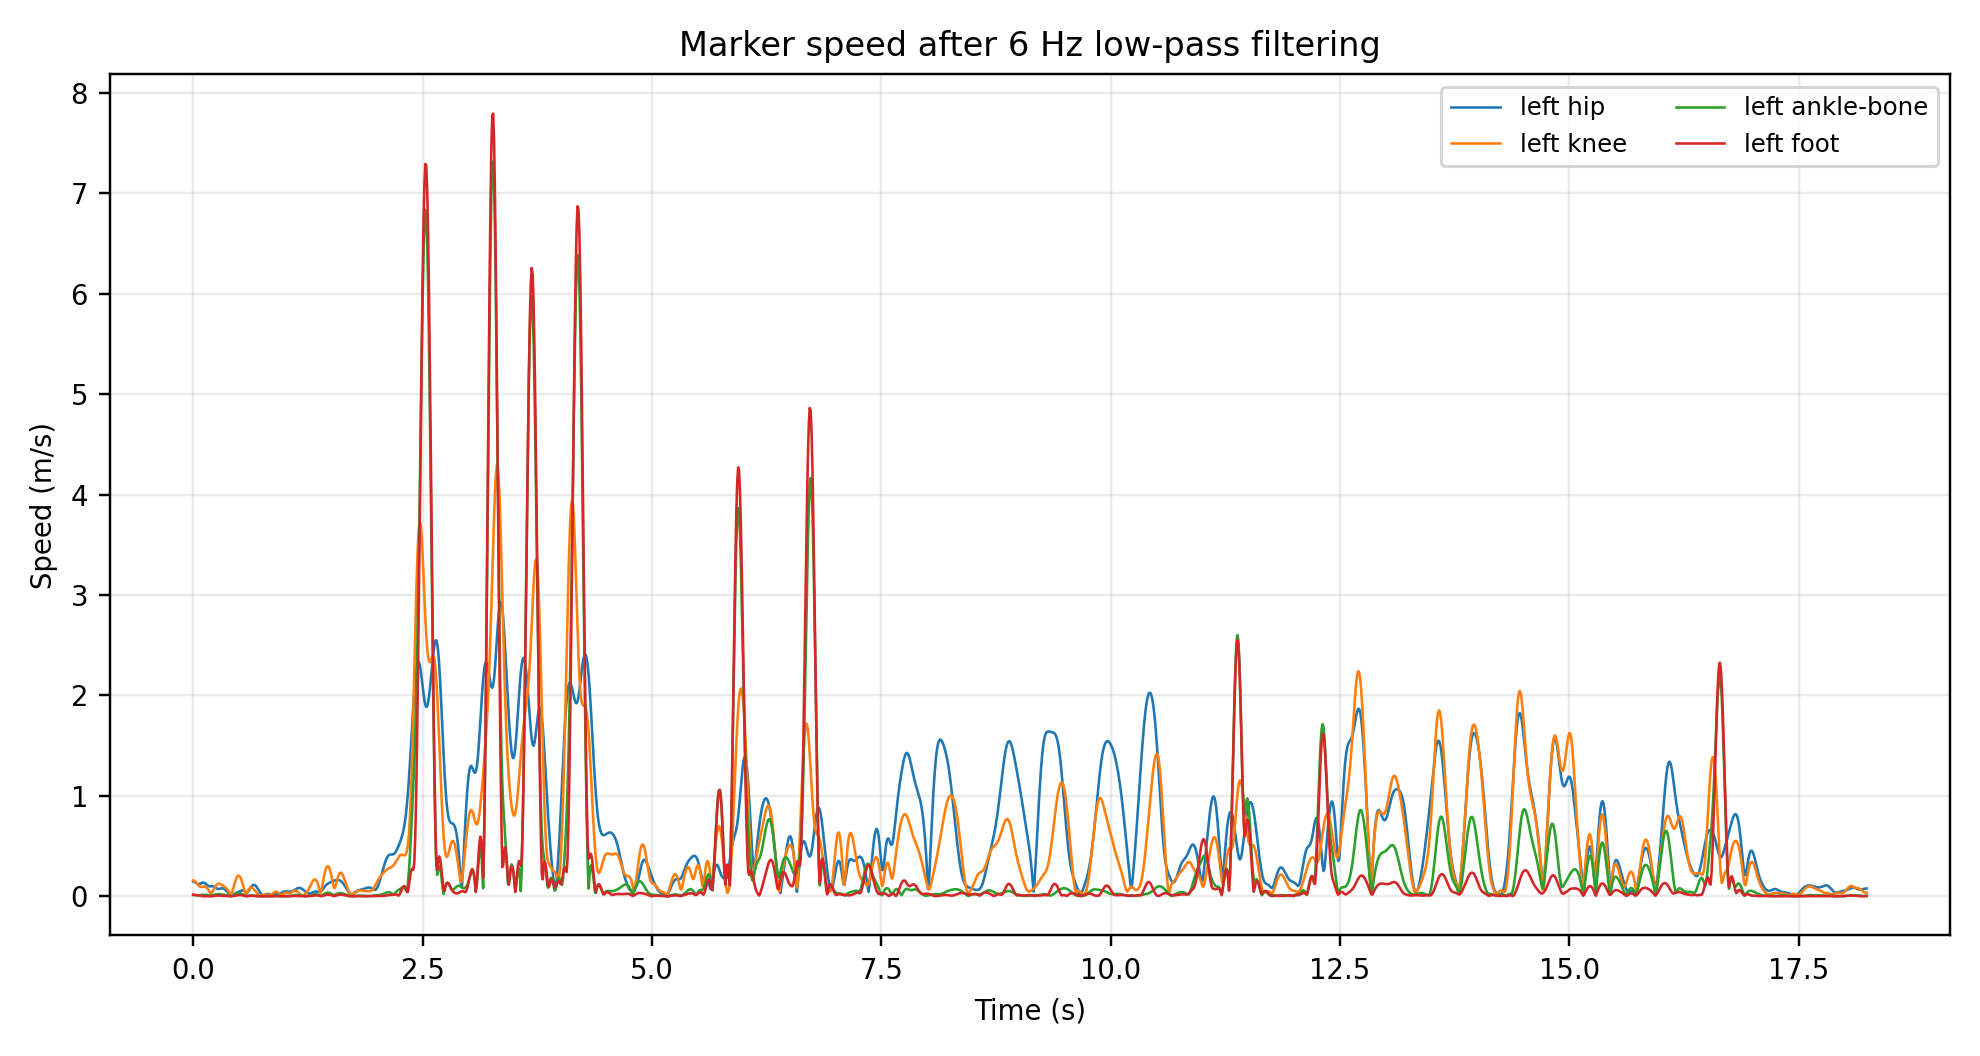
\includegraphics[width=0.92\textwidth]{marker_speed_time.png}
\caption{Marker speed magnitudes calculated by differentiating coordinates after fourth-order, zero-phase 6 Hz low-pass filtering.}
\label{fig:speed}
\end{figure}

\begin{table}[H]
\centering
\caption{Numerical derivative summaries. Values are computed outputs and should not be interpreted as valid physiological peaks until the trajectory discontinuities are resolved.}
\label{tab:speed}
\small
\begin{tabular}{lrrr}
\toprule
\textbf{Marker} & \textbf{Mean speed (m/s)} & \textbf{Peak speed (m/s)} & \textbf{Peak acceleration (m/s$^2$)} \\
\midrule
Left hip & 0.652 & 2.933 & 20.917 \\
Left knee & 0.576 & 4.287 & 41.980 \\
Left ankle-bone & 0.403 & 7.315 & 96.933 \\
Left foot & 0.351 & 7.792 & 105.010 \\
\bottomrule
\end{tabular}
\end{table}

\subsection{Inter-marker lengths}

Table~\ref{tab:lengths} and Figure~\ref{fig:lengths} summarise distances calculated between marker pairs. The distance variation is substantial: the hip--knee distance spans 37.6 mm, the knee--ankle distance spans 82.2 mm, and the ankle--foot distance spans 56.5 mm. These changes indicate that the marker coordinates do not behave as perfectly rigid anatomical segments throughout the trial. Soft-tissue motion can contribute to variation, but the magnitude and coincidence with abrupt framewise shifts mean tracking or reconstruction issues must also be considered.

\begin{figure}[H]
\centering
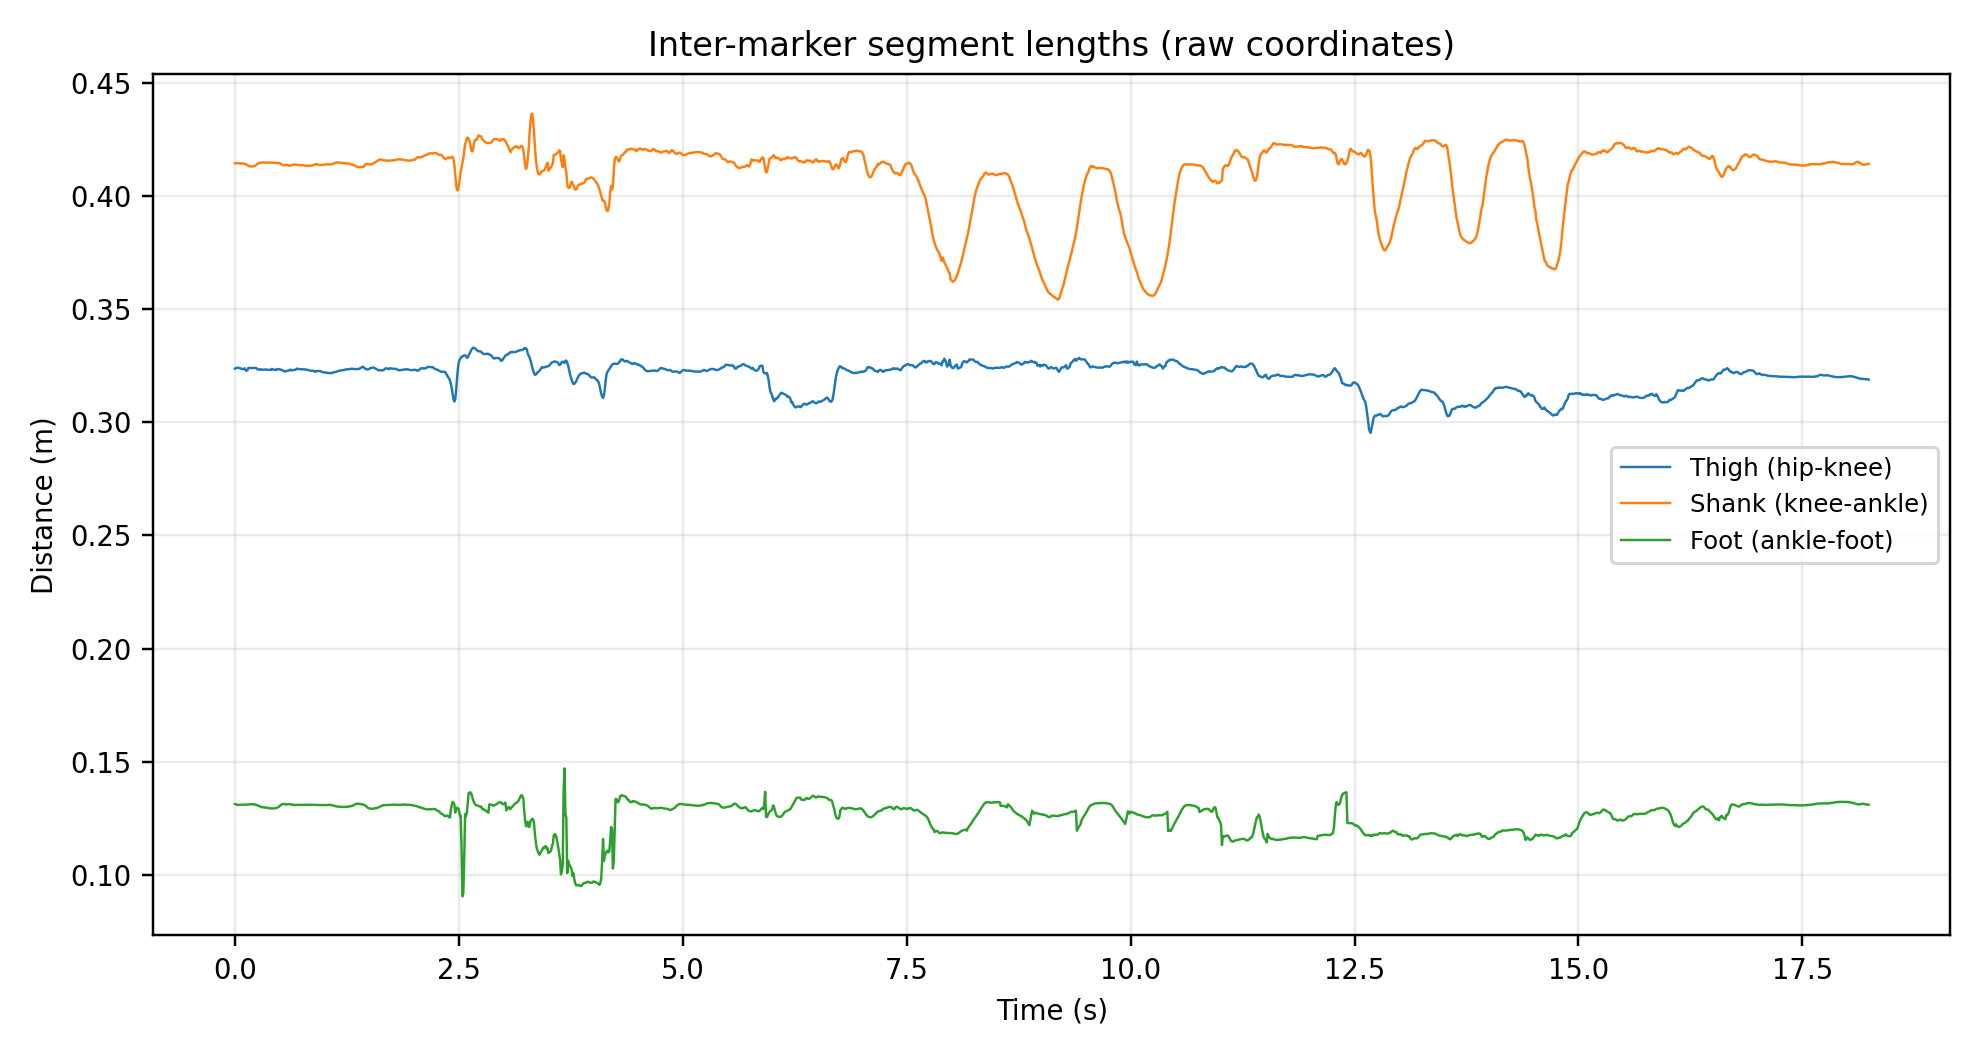
\includegraphics[width=0.92\textwidth]{segment_lengths_time.png}
\caption{Inter-marker distances computed from the raw coordinates. Large changes show that a rigid-segment assumption is not supported uniformly across this recording.}
\label{fig:lengths}
\end{figure}

\begin{table}[H]
\centering
\caption{Descriptive statistics of the raw inter-marker distances.}
\label{tab:lengths}
\small
\begin{tabular}{lrrrr}
\toprule
\textbf{Marker pair} & \textbf{Mean (m)} & \textbf{SD (m)} & \textbf{Minimum (m)} & \textbf{Maximum (m)} \\
\midrule
Hip--knee & 0.320 & 0.0067 & 0.295 & 0.333 \\
Knee--ankle & 0.409 & 0.0161 & 0.354 & 0.436 \\
Ankle--foot & 0.125 & 0.0074 & 0.091 & 0.147 \\
\bottomrule
\end{tabular}
\end{table}

\subsection{Secondary geometric angles calculated from C3D markers}

The filtered marker positions were used to compute a knee-flexion proxy and an unsigned ankle/shank--foot included angle. Figure~\ref{fig:angles} illustrates their variation. The calculated knee-flexion proxy ranges from $7.24^\circ$ to $127.34^\circ$ (range $120.10^\circ$). The ankle/shank--foot included angle ranges from $60.65^\circ$ to $133.86^\circ$ (range $73.21^\circ$).

\begin{figure}[H]
\centering
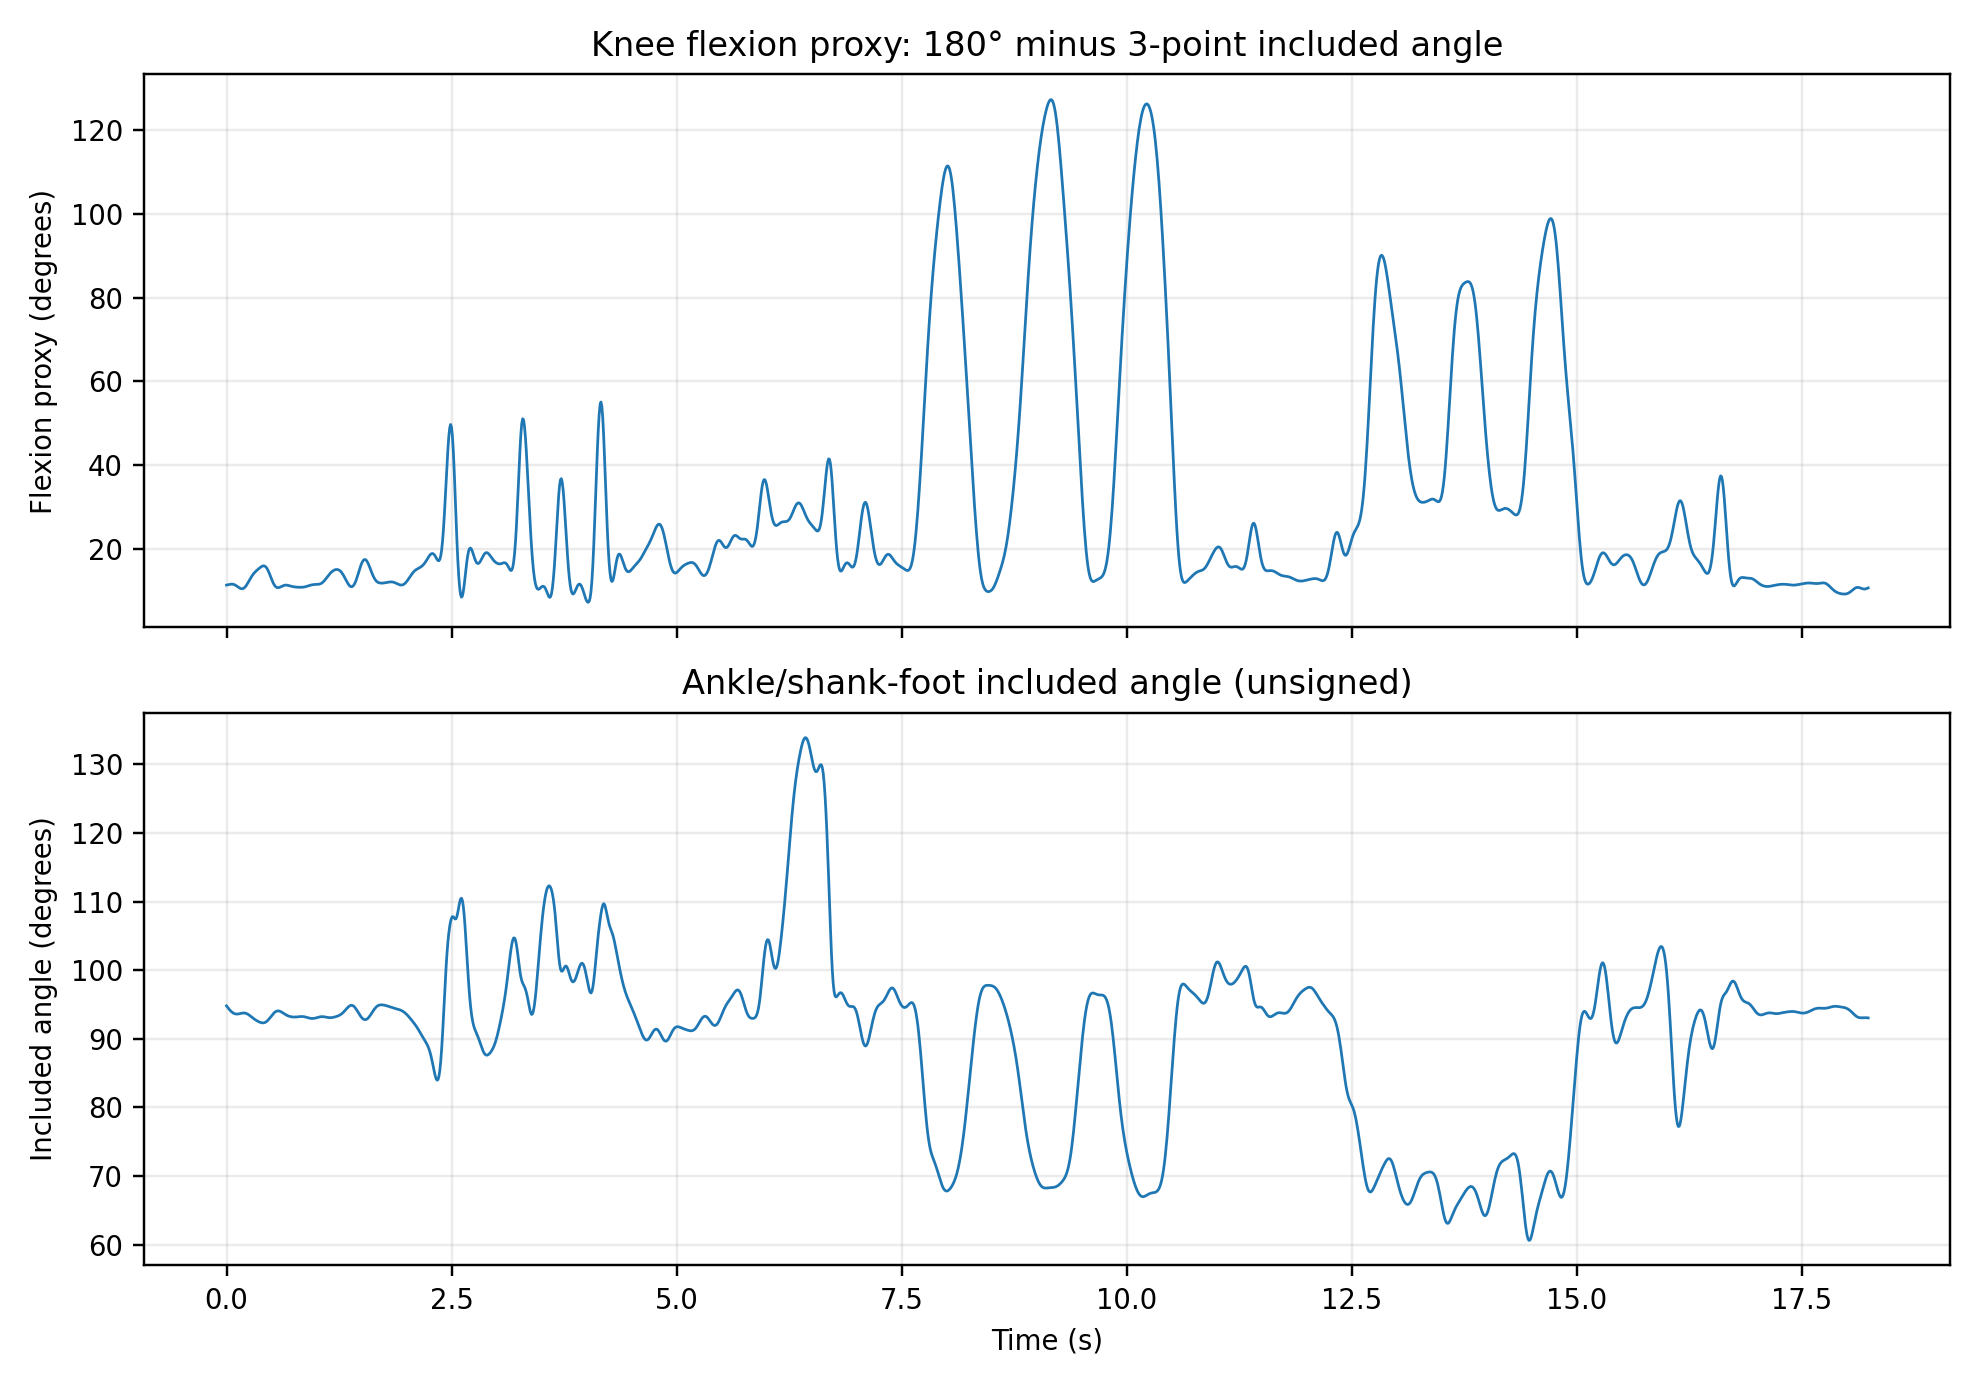
\includegraphics[width=0.92\textwidth]{joint_angles_time.png}
\caption{Marker-based geometric angle estimates from filtered trajectories. The ankle curve is an unsigned included angle, not a signed clinical dorsiflexion/plantarflexion measurement.}
\label{fig:angles}
\end{figure}

These coordinate-derived values are secondary geometric estimates only. Their ranges differ from the system-reported VMC values because they are based on four exported marker points and a simple dot-product definition, rather than the VMC system output and its own model/convention. The coordinate-derived angles should not be substituted for the VMC knee and ankle angles in the primary results.

\subsection{Visual Motion Capture joint-angle results reconstructed in MATLAB}

The primary knee and ankle angle results are taken from the angle outputs of the Visual Motion Capture system and reconstructed in MATLAB. The knee angle ranges from $151.31^\circ$ to $169.74^\circ$, giving a reported ROM of $18.43^\circ$. The ankle angle ranges from $76.08^\circ$ to $99.70^\circ$, giving a reported ROM of $23.62^\circ$. The reported peak angular velocities are $401.84^\circ/\mathrm{s}$ for the knee and $298.56^\circ/\mathrm{s}$ for the ankle; the corresponding reported peak absolute angular accelerations are $7274.19^\circ/\mathrm{s}^2$ and $19862.22^\circ/\mathrm{s}^2$. These metrics are attributed to the VMC/MATLAB angle workflow and are not recalculated from the C3D marker coordinates.

Figure~\ref{fig:vmc-range} visualises the reported VMC angle ranges. The supplied \file{VMC_joint_angles.csv} has no data rows, so this revision preserves the reported summary metrics but cannot independently regenerate the underlying VMC time-series curves from raw samples. The companion MATLAB script can recreate the angle trajectories and calculate the derivatives when the VMC angle export is saved as \file{VMC_joint_angles.csv}.

\begin{figure}[H]
\centering
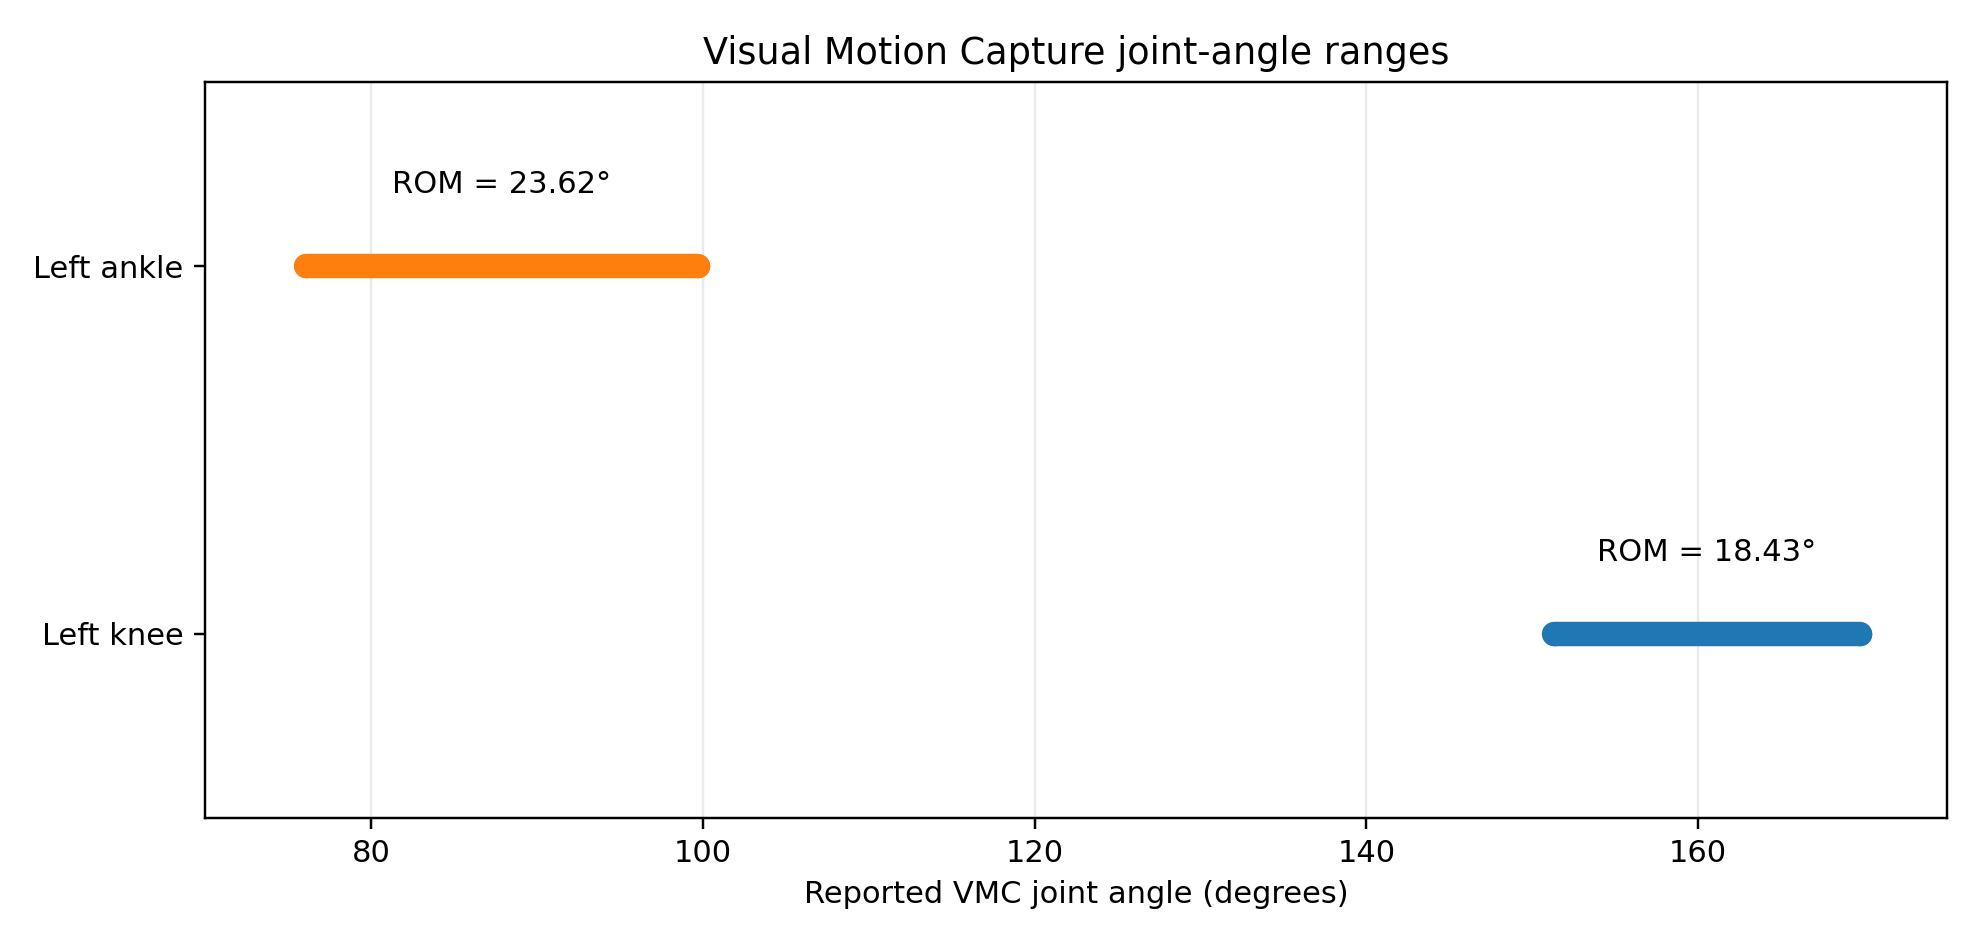
\includegraphics[width=0.82\textwidth]{vmc_joint_angle_ranges.png}
\caption{Minimum-to-maximum ranges of the VMC system joint angles, with ROM calculated as maximum minus minimum. These are summary ranges, not a reconstruction of the underlying time-series curves.}
\label{fig:vmc-range}
\end{figure}

\begin{table}[H]
\centering
\caption{VMC joint-angle metrics recorded in the original report draft and analysed in MATLAB.}
\label{tab:vmc-angles}
\small
\begin{tabular}{lrrrrr}
\toprule
\textbf{Joint} & \textbf{Min ($^\circ$)} & \textbf{Max ($^\circ$)} & \textbf{ROM ($^\circ$)} & \textbf{Peak $|\omega|$ ($^\circ$/s)} & \textbf{Peak $|\alpha|$ ($^\circ$/s$^2$)} \\
\midrule
Left knee & 151.31 & 169.74 & 18.43 & 401.84 & 7274.19 \\
Left ankle & 76.08 & 99.70 & 23.62 & 298.56 & 19862.22 \\
\bottomrule
\end{tabular}
\end{table}

\section{Discussion}

\subsection{Interpreting the two related data streams}

The Visual Motion Capture system supplied the primary knee and ankle angle series, which were reconstructed and analysed in MATLAB. The reported angular ranges and derivative summaries are distinct from the secondary geometric values calculated from C3D points. The supplied C3D file also provides four left-lower-limb marker trajectories across 1825 frames at 100 Hz, allowing an independent review of marker coordinates and inter-marker distances. Keeping these streams distinct avoids attributing the VMC angle convention to a separate geometric calculation.

\subsection{Limits to physiological interpretation}

The C3D point stream contains abrupt changes and substantial inter-marker length variation, which limit interpretation of coordinate-derived speed, acceleration, and marker-based geometric angles. They indicate that the coordinate export should be reviewed in the original VMC software and checked for trial concatenation, marker identity, axis transformation, or reconstruction problems. These findings do not, by themselves, invalidate the system-generated angle measurements. The VMC angle range and derivative values should be interpreted using the system angle convention and the MATLAB processing details, especially because numerical differentiation can amplify noise in the angle series.

The supplied C3D file reports zero analog channels used. No force plate, EMG, or other synchronized analog signal was available for corroboration. The file also contains no verified anatomical coordinate-system definition in the information used for this report. Thus, claims about ground contact, heel strike, joint moments, muscle activation, or signed ankle dorsiflexion/plantarflexion cannot be substantiated from this file alone.

\subsection{Recommended corrections to the experimental workflow}

Before drawing conclusions from the independent C3D coordinate derivatives, the raw trajectories should be checked in the motion-capture software around the large changes seen near 2.5--4.3 s and elsewhere in the coordinate plots. Confirm that point labels remain attached to the same physical markers, that the trial was not concatenated from separate capture segments, and that camera reconstruction and any gap-filling settings are appropriate. Re-export the corrected point trajectories and compare segment lengths across frames. This check applies to the C3D coordinate stream. The VMC-reported joint angles should retain the VMC system's defined angle convention; any newly calculated marker-based angles should be described separately unless the marker model and coordinate conventions are confirmed to be equivalent.

The supplied \file{VMC_joint_angles.csv} contains column headers only, and the MATLAB workspace was not provided. Accordingly, the angle summaries available in the original report draft are retained without independent recalculation, while the companion MATLAB script documents how to regenerate the time-series plots and derivative metrics from a populated VMC angle export. No unverified web-simulator performance claims are included.

\subsection{MATLAB reproducibility}

The companion MATLAB script \file{reconstruct_vmc_angles.m} reads a VMC angle export named \file{VMC_joint_angles.csv} with columns \file{Time_s}, \file{Knee_angle_deg}, and \file{Ankle_angle_deg}. It recreates time-series plots, calculates angular velocity and acceleration using numerical gradients, and exports a summary table. The supplied VMC CSV currently contains no sample rows; consequently, the current PDF contains the angle summary metrics recorded in the original draft and a range plot, rather than fabricated sample-by-sample curves estimated from only minimum and maximum values.

\section{Conclusion}

The practical combined Visual Motion Capture system angle outputs with MATLAB reconstruction and analysis. The primary reported knee angle ranged from $151.31^\circ$ to $169.74^\circ$ (ROM $18.43^\circ$), and the ankle angle ranged from $76.08^\circ$ to $99.70^\circ$ (ROM $23.62^\circ$). The reported angular velocity and acceleration summaries are separated from the independent C3D point calculations. The supplied C3D file was also decoded to examine four marker trajectories and calculate secondary coordinate-based kinematic estimates. Because the C3D point stream shows abrupt frame-to-frame changes and segment-length variation, those coordinate-derived quantities require a separate tracking/export-quality review. They should not be used to reject the VMC angle data automatically or to replace the joint angles measured by the capture system.

\end{document}
